\documentclass{report}

\usepackage[ngerman]{babel}
\usepackage[utf8]{inputenc}
\usepackage[T1]{fontenc}
\usepackage{hyperref}
\usepackage{csquotes}
\usepackage[a4paper]{geometry}
\usepackage{graphicx}

\usepackage[
    backend=biber,
    style=apa,
    sortlocale=de_DE,
    natbib=true,
    url=false,
    doi=false,
    sortcites=true,
    sorting=nyt,
    isbn=false,
    hyperref=true,
    backref=false,
    giveninits=false,
    eprint=false]{biblatex}
\addbibresource{../references/bibliography.bib}


\title{Ethik und Daten in der KI}
\author{Luka Adjancic}
\date{\today}

\parskip=2em
\parindent=1em
\renewcommand{\familydefault}{\sfdefault}

\begin{document}

\begin{figure}
    \centering
    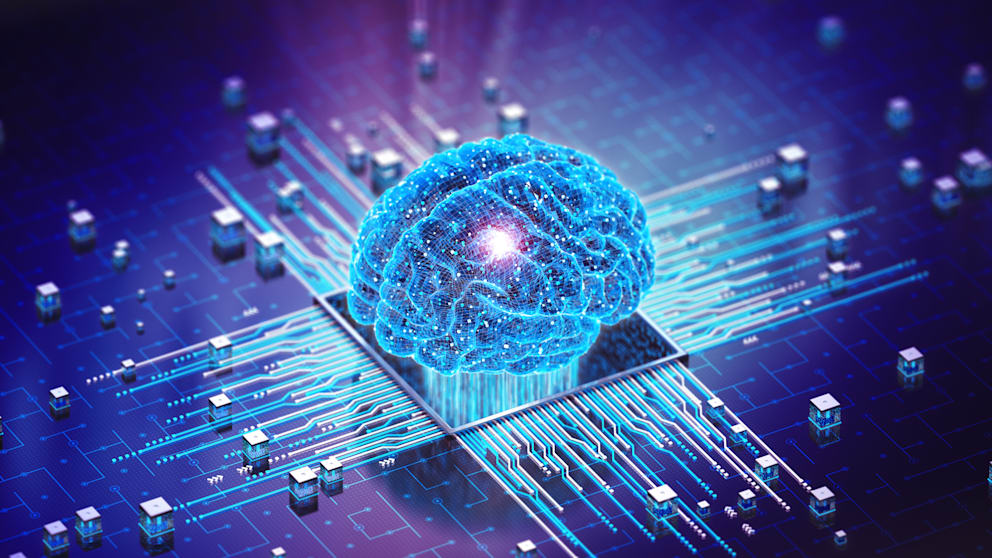
\includegraphics[width=1\textwidth]{AI.jpg}
    \caption{Künstliche Intelligenz als Bild dargestellt}
    \label{fig:AI}
\end{figure}

\maketitle

\tableofcontents

\chapter{Einleitung}

In diesem Dokument handelt es sich um das Thema Ethik und Daten. Ein grossteil dieser Fragen wurden mit einer KI beantwortet. Jedoch wurden bestimmte Fragen nicht nur von KI beantwortet, sondern auch von Mir. Das Dokument befasst sich mit der Ethik der KI und wie sie Daten speichert und verwendet. 

\chapter{Künstliche Intelligenz}
\label{chap:ai}

In diesem Kapitel wird die KI erklärt.

\section{Was ist KI?}

Künstliche Intelligenz ist ein Teilgebiet der Informatik, das sich mit der Entwicklung von Computersystemen befasst, die Aufgaben erfüllen können, die normalerweise menschliche Intelligenz erfordern. \textit{"KI wird weltweit für verschiedene militärische Aufgaben eingesetzt, um Prozesse zu optimieren und zu beschleunigen." \citep{ethics-ai-wikipedia}}\newline
KI existiert schon länger, jedoch war sie nicht so fortgeschritten wie heute. Vor ChatGPT gab keinen KI, welche in der Lage war Fragen und Text zu analysieren und auf diese Antworten zu geben. Dank Nvidia, ein Frima welche GPUs(Graphical Processing Unit) herstellt. Konnte OpenAI ChatGPT entwickeln.

\section{Wie analysiert KI Texte?}

KI analysiert Texte, indem sie Algorithmen nutzt, um aus riesigen Datensätzen Regeln abzuleiten oder Muster zu erkennen. Dies ermöglicht es, Verhaltensmuster oder -abweichungen zu erkennen, die die Grundlage für automatisierte Entscheidungen bilden. \textit{"Die Interpretation menschlicher Sprache durch Maschinen besitzt bei der KI-Forschung eine entscheidende Rolle. So ergeben sich etwaige Ergebnisse des Turing-Tests vor allem in Dialogsituationen, die bewältigt werden müssen." \citep{ai-wikipedia}}

\section{Vor- und Nachteile von KI}

Vorteile der KI sind eine hohe Reaktionsgeschwindigkeit und Genauigkeit, die Möglichkeit, große Informationsmengen schnell zu verarbeiten, die Reduzierung der menschlichen Kosten des Krieges und die Chance, Probleme zu lösen, die für Menschen aufgrund ihrer limitierten Kapazitäten schwer zu lösen sind. Nachteile der KI könnten sein, dass KI-Maschinen sich gegen die Interessen der Menschen wenden könnten und dass KI diskriminierend sein oder Vorurteile verstärken könnte. Es ist wichtig, dass der Einsatz von KI ethischen Grundsätzen folgt und die Würde des Menschen sowie Grundrechte respektiert.\newline
Die Nachteile der KI sind hauptsächlich diese rechnen mit Daten. \textit{"von Handlungen und Entscheidungen, die durch automatisierte/künstliche Intelligenz (KI) in Bezug auf Daten im Allgemeinen und personenbezogene Daten im Besonderen gesteuert werden" \citep{ethics-cognizant}} Obwohl die KI effizienter ist, kann sie nicht selber nachdenken. Ebenfalls hat die KI nicht so viel Speicherplatz für ihre Datenback, wie es Menschen haben. Für uns Menschen ist das Gehirn eine Art riesige Datenbank auf die wir zurückgreifen können.\newline
KI kann oft falsch liegen, weil Algorithmen für KI und maschinelles Lernen aus den Rückmeldungen der Nutzer lernen, basierend auf Trainingsdaten, die Verzerrungen enthalten können, wenn bestimmten Merkmalen und Eigenschaften der Vorzug gegeben wird. Dies kann zu Fehlern oder Lücken im Training führen, die dazu führen können, dass der KI falsches Verhalten beigebracht wird, das nicht mit menschlichen Werten vereinbar ist.

\begin{figure}[h]
    \centering
    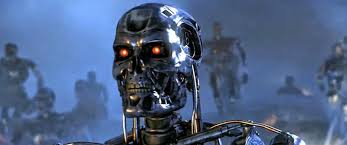
\includegraphics[width=0.5\textwidth]{rogue_ai.jpeg}
    \caption{Eine fiktionales Beispiel einer schlechten KI}
    \label{fig:rogueAI}
\end{figure}


\chapter{Ethik}
\label{chap:ethics}

In diesem Kapitel werde ich die Ethik im zusammenhang zur KI beschreiben.

\section{Was ist Ethik?}

thik ist jener Teilbereich der Philosophie, der sich mit den Voraussetzungen und der Bewertung menschlichen Handelns befasst. \textit{" Die (allgemeine) Ethik wird heute als die philosophische Disziplin verstanden, die Kriterien für gutes und schlechtes Handeln und für die Bewertung seiner Motive und Folgen aufstellt. Sie ist von ihrer Zielsetzung her eine praktische Wissenschaft." \citep{ethics-wikipedia}}

\section{Warum die KI schlecht und gut nicht unterscheiden kann}

Man unterscheidet zwischen richtig und falsch, indem man sich an bestimmte Werte und Gesetze hält. Zum Beispiel wird das Überqueren einer roten Ampel als falsch angesehen, da es gegen das Gesetz verstößt. Es geht also darum, sich an moralische und gesetzliche Normen zu halten, um zwischen richtigem und falschem Handeln zu unterscheiden. Für die KI ist egal ob etwas schlecht oder gut ist, weil es ihr so beigebracht wurde zu handeln, wenn man einer KI beibringt, dass töten gut sei. Diese KI würden dann glauben, dass diese Aussage stimmt und würde sie unter gar keinen Umständen hinterfragen, wie es Menschen machen würden.

\begin{figure}[h]
    \centering
    
\includegraphics[width=0.5\textwidth]{ethics.jpg}
    \caption{Ein Schild beschrieben mit richtig und falsch}
    \label{fig:ethics}
\end{figure}

\section{Das Trolley Problem}

Ein gutes Beispiel, bei welchem die KI probleme hätte. Das Trolley-problem ein sehr bekanntes Dilemma. Es handelt sich um sechs Personen, auf der einen Schiene sind fünf Personen, auf der abzweigung ist eine Person. Wenn jetzt eine KI, welche trainiert ist Menschen zu beschützen, in so einem Geschehen vorkommen würde. Das Trolley-Problem ist bekannt, weil den Hebel betätigen würde heissen, man hat dafür gesorgt das eine Person umgebracht wurde, jedoch ist man dann Schuld für diesen Tot. Ignoriert man das Geschehen werden fünf Personen umgebracht, man ist zwar nicht Schuld aber man hätte dies verhindern können. Eine KI hätte hier grosse Mühe oder würde denn logischten weg berechnen, der jedoch unmoralisch ist. \textit{"bei denen intuitiv die Rettung von fünf Menschen auf Kosten von einem Menschenleben unzulässig erscheint. Diese Erklärungslücke bezeichnet Judith Jarvis Thomson als Trolley-Problem und stellt dem Weichenstellerfall dazu" \citep{trolley-problem-wikipedia}}

\begin{figure}[h]
    \centering
    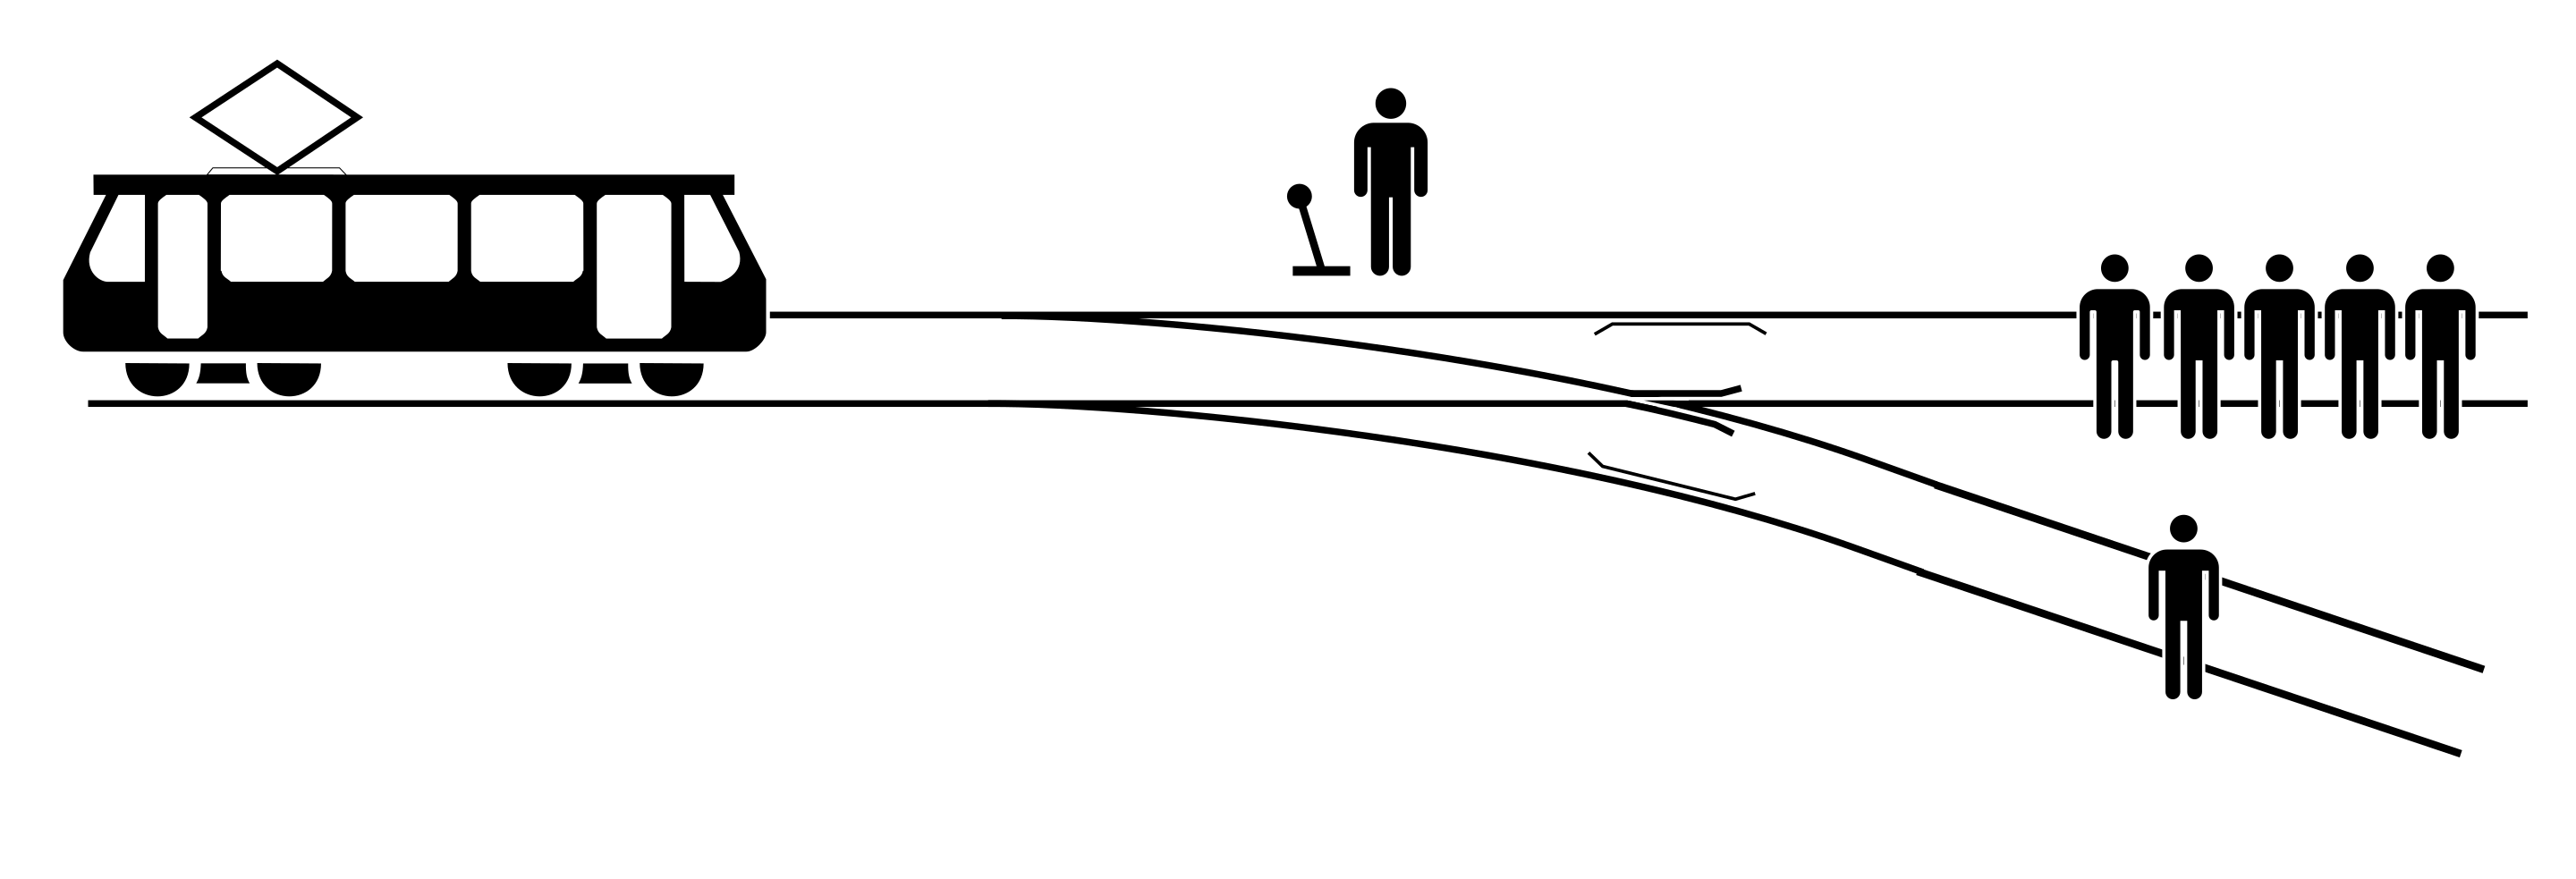
\includegraphics[width=0.5\textwidth]{Trolley_Problem.png}
    \caption{Das Trolley Problem}
    \label{fig:trolley_problem}
\end{figure}

\chapter{Daten}
\label{chap:data}

In diesem Kapitel werde ich die Daten beschreiben.

\section{Was sind Daten?}

Daten sind Informationen, die in eine Form übersetzt wurden, die für das Kopieren oder Verarbeiten effizient ist. In heutigen Computern und Übertragungsmedien sind Daten Informationen, die in eine binäre digitale Form umgewandelt wurden. \textit{"Gemäß Terminologie der geltenden Norm des internationalen Technologiestandards ISO/IEC 2382-1 für Informationstechnik (seit 1993) sind Daten – Data: „a reinterpretable representation of information in a formalized manner, suitable for communication, interpretation" \citep{data-wikipedia}} Sie werden in Computern als Bits oder Bytes gespeichert. 

\begin{figure}[h]
    \centering
    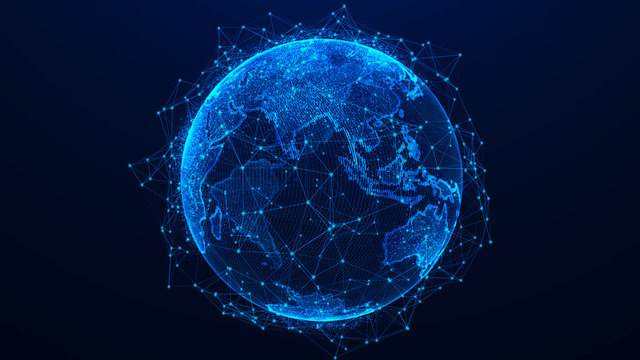
\includegraphics[width=0.5\textwidth]{data.jpg}
    \caption{Globale Daten verknüpft mit dem Internet}
    \label{fig:data}
\end{figure}

\section{Welche Daten werden geschützt?}

Die Arten von Daten, die durch die DSGVO geschützt sind, sind personenbezogene Daten wie Namen, Adressen, Telefonnummern, E-Mail-Adressen, etc. Diese Daten sind geschützt, um die Privatsphäre und die Rechte der betroffenen Personen zu wahren. Beispiele für geschützte Daten sind Kundendaten, Mitarbeiterdaten und Lieferantendaten. Es ist wichtig, diese Datenethik zu beachten, um das Vertrauen der Kunden zu gewinnen und zu erhalten. Durch Maßnahmen wie Datenverschlüsselung und Datenintegrität können Risiken wie Ransomware und Datenmanipulation minimiert werden, was wiederum das Vertrauen der Kunden stärkt. \textit{"Daten sind durch die DSGVO geschützt" \Citep{data-wbs}}

\section{Wie und warum werden Daten verkauft?}

Daten werden verkauft, indem Datenhändler sie an andere Unternehmen weitergeben, die sie für kommerzielle Zwecke nutzen. Datenhändler verkaufen Informationen wie persönliche Daten, Kaufverhalten, Interessen und andere relevante Informationen an Unternehmen, die diese Daten für ihre Marketing- und Geschäftsstrategien verwenden. Die Legalität des Handels mit Daten variiert von Land zu Land und die Rechtslage ist nicht immer eindeutig. Wenn Datenhändler ihre Informationen aus öffentlich zugänglichen Quellen beziehen, bewegen sie sich in der Regel auf der legalen Seite. \textit{"Neben den ethischen und juristischen Fragen, die der Datenhandel aufwirft, ist es das Ausmaß an Datenschutzverletzungen, das Anlass zur Sorge gibt. Datenhändler häufen vertrauliche Daten an, die in den falschen Händen für die Betroffenen schwerwiegende Konsequenzen haben können" \Citep{data-kaspersky}}

\printbibliography

\nocite{*}

\listoffigures

\end{document}
